\chapter{Технологический раздел}

В данном разделе делается выбор используемой СУБД и других средств реализации приложения, создаются триггер и ролевая модель в системе. Описывается создание пользовательского интерфейса.
Демонстрируется работа созданного приложения.

Ролевая модель создаётся на основе той, что была сформулирована в аналитическом разделе. Представляется код на языке Cypher для создания ролей, а также триггера.

\section{Выбор СУБД}

Самыми распространёнными~\cite{popular} СУБД графового типа являются \newline JanusGraph~\cite{janusgraph}, Neo4j~\cite{neo4j} и Dgraph~\cite{dgraph}.

\begin{enumerate}[label=\arabic*.]
	\item \textbf{JanusGraph}. Встроенный сложный поиск, а также дополнительная (опциональная) поддержка Elasticsearch. Использование полного по Тьюрингу языка запросов для обхода графов.
	\item \textbf{Neo4j}. Масштабируемость БД за счет разделения данных на части – сегменты. Высокий уровень безопасности: несколько экземпляров баз данных можно разделить, оставив их на одном выделенном сервере. Использование Cypher – языка запросов для графовых БД.
	\item \textbf{Dgraph}. Горизонтальная масштабируемость для работы в реальной среде с ACID-транзакциями. Использование языка запросов GraphQL.
\end{enumerate}

В данной работе используется Neo4j, так как эта СУБД предоставляет достаточный инструментарий для реализации поставленных задач.

\section{Выбор средств реализации}

В качестве языка программирования для реализации программного продукта был выбран Python~\cite{python}. 
Для взаимодействия с СУБД используется библиотека neo4j~\cite{pythonwithneo4j}, которая, как и другие python-библиотеки, устанавливается с помощью встроенного в python пакетного менеджера pip.
Также в СУБД Neo4j используется дополнительный плагин APOC~\cite{apoc}, предоставляющий необходимый набор процедур для работы с Neo4j, одной из которых является процеудра регистрации нового триггера.

\section{Создание базы данных}

В данной работе требуется задать ролевую модель на основе разработанной в аналитическом разделе и создать удаляющий триггер.

\textbf{Создание ролевой модели}

В конструкторском разделе была разработана следующая ролевая модель:
\begin{enumerate}[label=\arabic*.]
	\item doctor --- психолог. Имеет все права над всеми таблицами;
	\item patient --- пациент. Имеет доступ SELECT ко всем таблицам;
	\item family --- родственник. Имеет доступ SELECT и UPDATE ко всем таблицам.
\end{enumerate}

Сценарий создания ролей представлен в Листинге \ref{roles}.
\begin{center}
	\begin{lstlisting}[label=roles, caption=Создание ролевой модели]
CREATE ROLE doctor
CREATE ROLE patient
CREATE ROLE family
GRANT MATCH {*} ON GRAPH dictionary to doctor
GRANT WRITE ON GRAPH dictionary to doctor
GRANT MATCH {*} ON GRAPH dictionary to patient
GRANT MATCH {*} ON GRAPH dictionary to family
GRANT SET PROPERTY {*} ON GRAPH dictionary to family
GRANT SET LABEL {*} ON GRAPH dictionary to family
\end{lstlisting}
\end{center}

\textbf{Создание триггера}

Сценарий создания триггера представлен в Листинге \ref{apoc}.
\begin{center}
	\begin{lstlisting}[label=apoc, caption=Создание триггера]
CALL apoc.trigger.add('deleteOrphanedNodes', 'UNWIND $deletedNodes AS dn MATCH (n) WHERE NOT ()-[:own]->(n) AND NOT n:owner DETACH DELETE n' , {phase: 'after'})
\end{lstlisting}
\end{center}

\pagebreak

\section{Интерфейс взаимодействия}

Для работы с БД создан API с помощью библиотеки fastapi~\cite{fastapi}. 
В программном интерфейсе реализованы методы для выполнения операций создания, чтения, обновления и удаления узлов в базе данных.
На рисунке \ref{fastapi} представлена часть имеющихся методов, таких как:
\begin{enumerate}
	\item создать:
		\begin{enumerate}[label=\alph*.]
			\item термин;
			\item действие объекта;
			\item действие субъекта;
		\end{enumerate}
	\item получить:
	\begin{enumerate}[label=\alph*.]
		\item все узлы;
		\item все термины владельца;
		\item все термины;
	\end{enumerate}
	\item изменить:
	\begin{enumerate}[label=\alph*.]
		\item термин;
		\item действие объекта;
		\item декйствие субъекта;
	\end{enumerate}
	\item удалить:
	\begin{enumerate}[label=\alph*.]
		\item термин;
		\item действие объекта;
		\item действие субъекта.
	\end{enumerate}
\end{enumerate}

\begin{figure}[ht!]\centering
	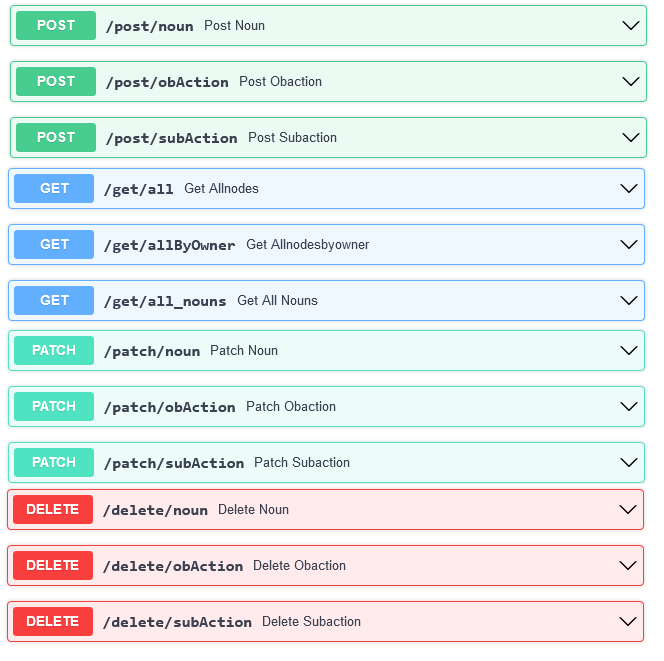
\includegraphics[scale=0.5]{smallapi}
	\caption{Программный интерфейс}
	\label{fastapi}
\end{figure}

\pagebreak

\section{Демонстрация работы}

На рисунке \ref{app} демонстрируется процесс получения ответа на запрос о получении всех возможных узлов в базе данных. Данный запрос требует на вход единственный параметр --- роль. Результатом запроса является JSON объект с параметрами status --- состояние запроса, results --- количество полученных узлов и nodes --- сами узлы. Результат отображён в нижней части рисунка \ref{app}.

\begin{figure}[ht!]\centering
	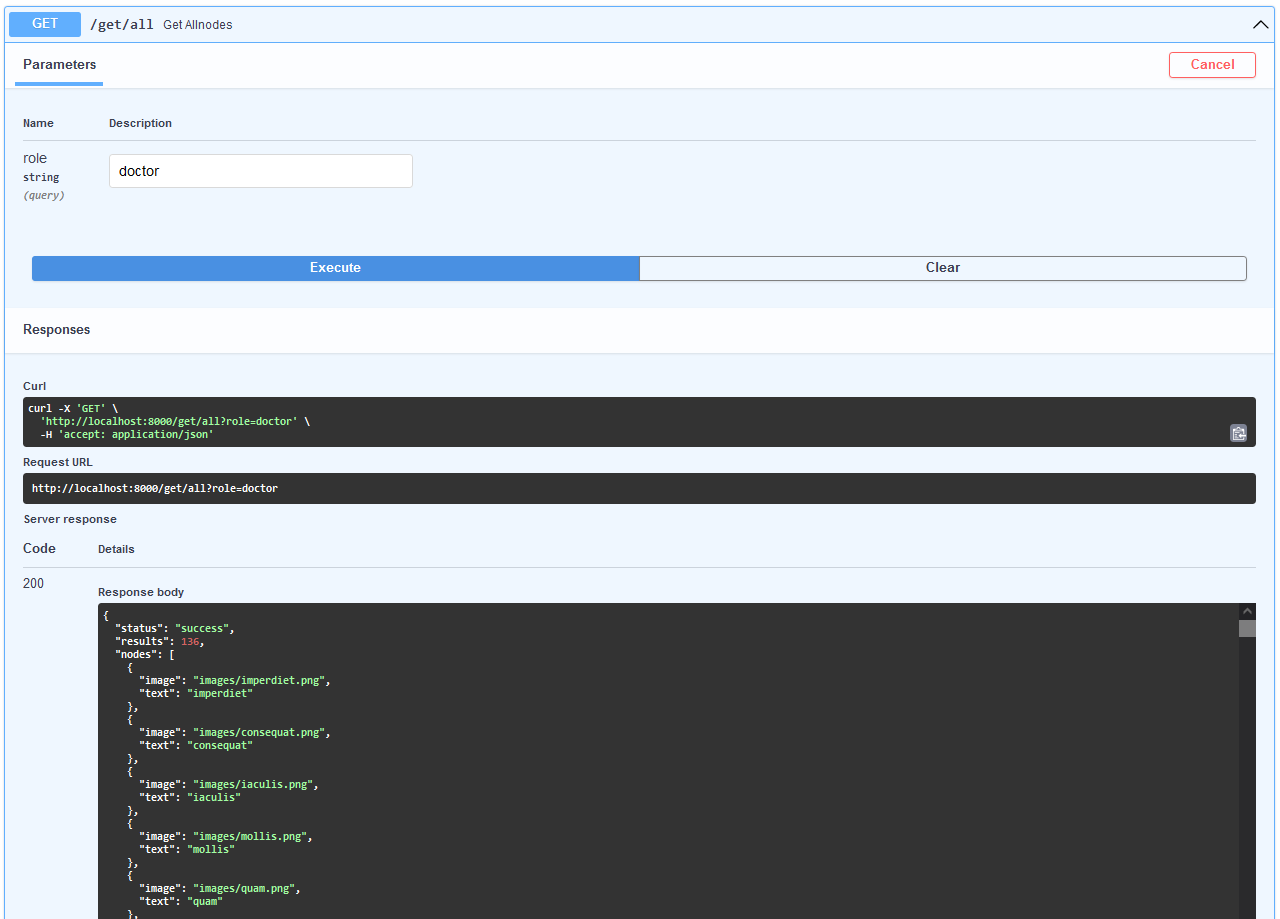
\includegraphics[scale=0.4]{app}
	\caption{Демонстрация работы программы}
	\label{app}
\end{figure}

\pagebreak

\section*{Вывод}

В данном разделе выбраны СУБД и средства реализации, представлено создание ролевой модели и триггера. Описан пользовательский интерфейс.

